% ---------------------------------------------------------------- 22 Ladder design
\begin{frame}{The context ladder}
  \small
  TomoSAR theory inverts the \emph{expected} covariance per pixel; no estimator is
  per-pixel in the data. Every practical route --- the GT's own Capon included --- buys
  that expectation with a spatial window over the stack vectors $\mathbf{g} \in \mathbb{C}^{N}$:
  \begin{center}
  \vspace{-2pt}
  \begin{tabular}{ccc}
    {\scriptsize\color{soft} theory: one pixel, in expectation} & &
    {\scriptsize\color{soft} practice: $w_{a}{\times}w_{r}$ boxcar $B(x)$ (az${\times}$rg)} \\[3pt]
    $\mathbf{R}(x) \;=\; \mathrm{E}\big[\mathbf{g}(x)\,\mathbf{g}^{\mathsf H}(x)\big]$ &
    \quad$\longrightarrow$\quad &
    $\hat{\mathbf{R}}(x) \;=\; \dfrac{1}{w_{a}w_{r}} \displaystyle\sum_{x' \in B(x)} \mathbf{g}(x')\,\mathbf{g}^{\mathsf H}(x')$ \\
  \end{tabular}
  \vspace{-2pt}
  \end{center}
  \begin{center}
  \vspace{12pt}
  \begin{columns}[c,totalwidth=0.98\textwidth]
    \begin{column}{0.06\textwidth}
    \end{column}
    \begin{column}{0.60\textwidth}
      \centering
      \begin{tikzpicture}
        \node[box, text width=22mm] (mlp) at (0,0)   {\textbf{pixel MLP}\\{\tiny $1{\times}1$ --- one look}};
        \node[box, text width=22mm] (c09) at (2.8,0) {\textbf{CNN small}\\{\tiny $9{\times}9$ --- inside $B(x)$}};
        \node[box, fill=accent!16, text width=22mm] (c29) at (5.6,0) {\textbf{CNN big}\\{\tiny $29{\times}29$ --- holds $B(x)$}};
        \draw[flow] (mlp) -- (c09);
        \draw[flow] (c09) -- (c29);
      \end{tikzpicture}
    \end{column}
    \begin{column}{0.32\textwidth}
      \centering
      \begin{tikzpicture}[scale=0.86]
        \draw[black!7, step=0.08] (-1.32,-1.32) grid (1.32,1.32);
        \draw[ink, thin] (-1.16,-1.16) rectangle (1.16,1.16);
        \node[font=\tiny, text=ink, anchor=south west, inner sep=1pt] at (-1.15,1.17) {$29{\times}29$};
        \fill[accent!16] (-1.04,-0.48) rectangle (1.04,0.48);
        \draw[accent, semithick, dashed] (-1.04,-0.48) rectangle (1.04,0.48);
        \draw[good, thin] (-0.36,-0.36) rectangle (0.36,0.36);
        \draw[good, thin] (0,0.36) -- (0,0.60);
        \node[font=\tiny, text=good, anchor=south, inner sep=1pt] at (0,0.60) {$9{\times}9$};
        \fill[accent] (-0.04,-0.04) rectangle (0.04,0.04);
        \node[font=\tiny, text=accent, anchor=north, inner sep=3pt] at (0,-0.05) {$1{\times}1$};
        \draw[accent, thin] (1.06,-0.62) -- (1.50,-1.05);
        \node[font=\tiny, text=accent, anchor=north west, inner sep=1pt] at (1.42,-1.02) {$B(x)$};
      \end{tikzpicture}
    \end{column}
  \end{columns}
  \vspace{-15pt}
  \begin{columns}[t,totalwidth=0.98\textwidth]
    \begin{column}{0.06\textwidth}
    \end{column}
    \begin{column}{0.60\textwidth}
      \raggedright
      {\scriptsize to scale: $9{\times}9$ sits \emph{inside} the label's window;
       $29{\times}29$ is the first field to swallow it. One trunk, no downsampling,
       \textbf{capacity held at ${\sim}31$\,M} on every rung --- the receptive field
       is the only thing that moves.\par}
    \end{column}
    \begin{column}{0.32\textwidth}
    \end{column}
  \end{columns}
  \end{center}
\end{frame}

% ---------------------------------------------------------------- 22b Why the ladder must help
\begin{frame}{Why the ladder must help --- the label is a window statistic}
  \setlength{\abovedisplayskip}{4pt}
  \setlength{\belowdisplayskip}{4pt}
  \small
  \setlength{\arrayrulewidth}{0.3pt}
  \arrayrulecolor{soft!60}
  \vspace{12pt}
  \begin{tabular}{@{}p{0.437\textwidth}@{\hspace{15pt}}|@{\hspace{17pt}}p{0.437\textwidth}@{}}
    \textbf{1. The label is $B(x)$-measurable.} Capon and the parameter fit are
    deterministic maps, so
    \[
      y(x) \;=\; \Phi\big(\mathbf{g}_{B(x)}\big),
    \]
    exactly, by construction --- no assumption on the scene. The label holds no
    randomness the looks in $B(x)$ do not already hold.
    \rule[-16pt]{0pt}{0pt}%
    &
    \textbf{2. The error splits into a floor and a fit.} For \emph{any} predictor
    $\hat y$ built from a field $\mathcal{F}$,
    \[
      \begin{aligned}
        \mathrm{E}\big[(y - \hat y)^{2}\big] = {}
          & \mathrm{E}\big[\mathrm{Var}(y \mid \mathbf{g}_{\mathcal{F}})\big] \\[2pt]
          & + \mathrm{E}\big[(\mathrm{E}[y \mid \mathbf{g}_{\mathcal{F}}] - \hat y)^{2}\big].
      \end{aligned}
    \]
    The first term is the \textbf{floor}, fixed by $\mathcal{F}$ alone; the second is
    what training buys.
    \rule[-16pt]{0pt}{0pt}%
    \\
    \hline
    \rule{0pt}{24pt}%
    \textbf{3. The floor only falls.} Take any two rungs with $\mathcal{F}_{1}
    \subseteq \mathcal{F}_{2}$ and condition once more on the wider one:
    \[
      \begin{aligned}
        \mathrm{Var}(y \mid \mathbf{g}_{\mathcal{F}_1}) = {}
          & \mathrm{E}\big[\mathrm{Var}(y \mid \mathbf{g}_{\mathcal{F}_2}) \mid \mathbf{g}_{\mathcal{F}_1}\big] \\[2pt]
          & + \mathrm{Var}\big(\mathrm{E}[y \mid \mathbf{g}_{\mathcal{F}_2}] \mid \mathbf{g}_{\mathcal{F}_1}\big).
      \end{aligned}
    \]
    The last term is a variance, hence $\ge 0$:
    \[
      \mathrm{E}\big[\mathrm{Var}(y \mid \mathbf{g}_{\mathcal{F}_1})\big]
      \;\ge\;
      \mathrm{E}\big[\mathrm{Var}(y \mid \mathbf{g}_{\mathcal{F}_2})\big].
    \]
    &
    \rule{0pt}{24pt}%
    \textbf{4. And it vanishes.} Once the field holds the whole window, the label's
    own looks are among those handed to the model:
    \[
      \begin{aligned}
        B(x) \subseteq \mathcal{F}
          &\;\Longrightarrow\; \mathbf{g}_{B(x)} \subseteq \mathbf{g}_{\mathcal{F}} \\[1pt]
          &\;\Longrightarrow\; y = \Phi(\mathbf{g}_{B(x)}) \text{ fixed by } \mathbf{g}_{\mathcal{F}} \\[1pt]
          &\;\Longrightarrow\; \mathrm{Var}(y \mid \mathbf{g}_{\mathcal{F}}) = 0.
      \end{aligned}
    \]
    \\
  \end{tabular}
\end{frame}

% ---------------------------------------------------------------- 22c The bottom rung
\begin{frame}{The floor of any field --- the fluctuation of the looks it misses}
  \begin{columns}[c]
    \begin{column}{0.47\textwidth}
      \small
      \setlength{\abovedisplayskip}{11pt}
      \setlength{\belowdisplayskip}{22pt}
      Take \emph{any} field $\mathcal{F}$ and split the label's window into the
      looks the field delivers and the looks it misses:
      \[
        w_{a}w_{r}\,\hat{\mathbf{R}}(x) \;=\; \left\{
        \begin{aligned}
          & \sum_{p \in B(x) \cap \mathcal{F}} \mathbf{g}(p)\mathbf{g}^{\mathsf H}(p) \\[2pt]
          & + \sum_{p \in B(x) \setminus \mathcal{F}} \mathbf{g}(p)\mathbf{g}^{\mathsf H}(p).
        \end{aligned}
        \right.
      \]
      The first sum is delivered, the second is missed. Which pixels fall in which
      is the \emph{only} thing that changes along the ladder.
      Condition on $\mathbf{g}_{\mathcal{F}}$. Every look in the first sum is one
      the field hands over, so that term is a constant and carries no variance ---
      only the misses fluctuate:
    \end{column}
    \begin{column}{0.47\textwidth}
      \small
      \setlength{\abovedisplayskip}{11pt}
      \setlength{\belowdisplayskip}{22pt}
      \[
        \begin{aligned}
          &\mathrm{Var}\big(\hat{\mathbf{R}}(x) \,\big|\, \mathbf{g}_{\mathcal{F}}\big) \\[5pt]
          &\quad = \mathrm{Var}\bigg(\frac{1}{w_{a}w_{r}}\sum_{p \in B(x) \cap \mathcal{F}} \mathbf{g}(p)\mathbf{g}^{\mathsf H}(p) \\[2pt]
          &\qquad\qquad + \frac{1}{w_{a}w_{r}}\sum_{p \in B(x) \setminus \mathcal{F}} \mathbf{g}(p)\mathbf{g}^{\mathsf H}(p)
            \,\bigg|\, \mathbf{g}_{\mathcal{F}}\bigg) \\[5pt]
          &\quad = \boxed{\;\frac{1}{(w_{a}w_{r})^{2}}\,\mathrm{Var}\bigg(
            \sum_{p \in B(x) \setminus \mathcal{F}} \mathbf{g}(p)\mathbf{g}^{\mathsf H}(p)
            \,\bigg|\, \mathbf{g}_{\mathcal{F}}\bigg)\;}
        \end{aligned}
      \]
      Exact: no assumption on the scene, no independence between looks. And when
      $B(x) \setminus \mathcal{F} = \varnothing$ the sum is empty --- the floor is
      $0$.
    \end{column}
  \end{columns}
\end{frame}

% ---------------------------------------------------------------- 22d The three rungs
\begin{frame}{The three rungs --- only one term moves}
  \vfill
  \begin{center}
  {\small
  \renewcommand{\arraystretch}{1.8}
  \setlength{\tabcolsep}{10pt}
  \begin{tabular}{@{}l c c c@{}}
    \toprule
      & \textbf{pixel MLP} & \textbf{CNN small} & \textbf{CNN big} \\
      & $r = 1$
      & $r < w_{r}$
      & $r \ge w_{a}$ \\
    \midrule
    misses $\big|B(x) \setminus \mathcal{F}\big|$
      & $w_{a}w_{r} - 1$
      & $w_{a}w_{r} - r^{2}$
      & $0$ \\
    \rowcolor{argA!22}
    label variance $\mathrm{E}\big[\mathrm{Var}(y \mid \mathbf{g}_{\mathcal{F}})\big]$
      & the misses fluctuate
      & the misses fluctuate
      & $\mathbf{0}$ \\
    model error $\mathrm{E}\big[(\mathrm{E}[y \mid \mathbf{g}_{\mathcal{F}}] - \hat y)^{2}\big]$
      & training buys
      & training buys
      & training buys \\
    \midrule
    total $\mathrm{E}\big[(y - \hat y)^{2}\big]$
      & floor $+$ model
      & floor $+$ model
      & \textbf{model alone} \\
    \bottomrule
  \end{tabular}}
  \end{center}
  \vspace{6pt}
  {\footnotesize\raggedright Every column is the same quantity,
   $w_{a}w_{r} - \big|B(x) \cap \mathcal{F}\big|$ --- the control meets the window in
   a single pixel, the small CNN in all $r^{2}$ of its field, the big CNN in the whole
   of it. Only the shaded row moves, and no architecture or loss touches it; model
   error reads the same in every column, and capacity is held fixed across the ladder,
   so the field is the only variable.
   \par}
  \vfill
\end{frame}

% ---------------------------------------------------------------- 23 Ladder result
\begin{frame}{Ladder result: context grounds the prediction}
  \centering
  \scriptsize
  \renewcommand{\arraystretch}{1.02}
  \setlength{\tabcolsep}{6pt}
  \begin{tabular}{@{}l c r@{\hskip 6pt}l r@{\hskip 6pt}l@{}}
    \toprule
    metric & pixel MLP & \multicolumn{2}{c}{CNN small \; ($\Delta$)} & \multicolumn{2}{c@{}}{CNN big \; ($\Delta$)} \\
    {\color{soft} field $\mathcal{F}$ / looks seen}
      & {\color{soft} $1{\times}1$ / $1$}
      & \multicolumn{2}{c}{\color{soft} $9{\times}9$ / $81$}
      & \multicolumn{2}{c@{}}{\color{soft} $29{\times}29$ / $312$} \\
    \midrule
    curve $R^2$ $\uparrow$                   & 0.24    & 0.47           & \hlval{good}{$+0.23$}    & \textbf{0.59}  & \hlval{good}{$+0.12$}  \\
    per-pixel $R^2$ (median) $\uparrow$      & \hlval{accent}{$-0.03$} & 0.42           & \hlval{good}{$+0.45$}    & \textbf{0.57}  & \hlval{good}{$+0.15$}  \\
    \addlinespace
    SSIM elevation $\uparrow$                & 0.918   & 0.949          & \hlval{good}{$+0.031$}   & 0.958 & \hlval{good}{$+0.009$} \\
    SSIM range $\uparrow$                    & 0.869   & 0.917          & \hlval{good}{$+0.048$}   & \textbf{0.928} & \hlval{good}{$+0.011$} \\
    SSIM azimuth $\uparrow$                  & 0.895   & 0.934          & \hlval{good}{$+0.039$}   & \textbf{0.944} & \hlval{good}{$+0.010$} \\
    peak error median [units] $\downarrow$   & 2.01    & \textbf{0.67}  & \hlval{good}{$-1.34$}    & \textbf{0.67}  & \textcolor{soft}{$0.00$}   \\
    \addlinespace
    matched recall $\uparrow$                & 0.61    & \textbf{0.69}  & \hlval{good}{$+0.08$}    & 0.68           & \hlval{accent}{$-0.01$} \\
    \quad 2 scatterers $\uparrow$            & 0.55    & 0.63           & \hlval{good}{$+0.08$}    & \textbf{0.70}  & \hlval{good}{$+0.06$}  \\
    count exact $\uparrow$                   & 0.56    & \textbf{0.68}  & \hlval{good}{$+0.12$}    & 0.62           & \hlval{accent}{$-0.06$} \\
    \addlinespace
    matched $\mu$ MAE [units] $\downarrow$   & 3.37    & 2.37           & \hlval{good}{$-1.00$}    & \textbf{2.12}  & \hlval{good}{$-0.25$}  \\
    \quad 2 scatterers $\downarrow$          & 5.70    & 4.30           & \hlval{good}{$-1.41$}    & \textbf{3.79}  & \hlval{good}{$-0.51$}  \\
    matched $\sigma$ MAE $\downarrow$        & 1.21    & 0.86           & \hlval{good}{$-0.35$}    & \textbf{0.84}  & \hlval{good}{$-0.02$}  \\
    \quad 2 scatterers $\downarrow$          & 2.01    & 1.59           & \hlval{good}{$-0.42$}    & \textbf{1.49}  & \hlval{good}{$-0.10$}  \\
    matched $a$ MAE $\downarrow$             & 0.531   & \textbf{0.326} & \hlval{good}{$-0.205$}   & 0.334          & \hlval{accent}{$+0.008$} \\
    \bottomrule
  \end{tabular}
  \par\smallskip
  \parbox{0.82\textwidth}{\tiny\color{soft} \textbf{runs}: conv head $\cdot$ sorted-GT $\cdot$ $K{=}2$ $\cdot$ param-MSE $\cdot$ active-norm $\cdot$ no aug (model = column).
   Looks seen out of $|B(x)| = w_{a}w_{r} = 26 \times 12 = 312$.
   Held-out test, $5.0$\,M px; \textbf{bold} = best, marked only where best and worst differ by more than $5\%$;
   $\Delta$ vs previous tier (\textcolor{good}{better} / \textcolor{accent}{worse}); \textcolor{accent}{red value} $=$ the $1{\times}1$ control regressing its conditional mean\par}
    

\end{frame}

% ---------------------------------------------------------------- 24b Correlation law
\begin{frame}{The correlation law --- how labels share their inputs}
  \setlength{\abovedisplayskip}{3pt}
  \setlength{\belowdisplayskip}{3pt}
  \begin{columns}[c,onlytextwidth]
    \begin{column}{0.46\textwidth}
      \centering
      {\scriptsize\textbf{Azimuth}: slide the second window along track.\par}
      \vspace{1pt}
      \begin{tikzpicture}[scale=0.80]
        \fill[accent!30] (0.42,1.95) rectangle (0.90,2.35);
        \draw[accent, thick] (0.10,1.95) rectangle ++(0.8,0.4);
        \draw[good, thick]   (0.42,1.95) rectangle ++(0.8,0.4);
        \node[font=\tiny, anchor=south] at (0.66,2.42) {$\tau_{a} = 0.4\,w_{a}$};
        \fill[accent!30] (2.94,1.95) rectangle (3.10,2.35);
        \draw[accent, thick] (2.30,1.95) rectangle ++(0.8,0.4);
        \draw[good, thick]   (2.94,1.95) rectangle ++(0.8,0.4);
        \node[font=\tiny, anchor=south] at (3.02,2.42) {$\tau_{a} = 0.8\,w_{a}$};
        \draw[accent, thick] (4.50,1.95) rectangle ++(0.8,0.4);
        \draw[good, thick]   (5.54,1.95) rectangle ++(0.8,0.4);
        \node[font=\tiny, anchor=south] at (5.42,2.42) {$\tau_{a} = 1.3\,w_{a}$};
        \draw[soft, dashed, thin] (0.66,1.90) -- (1.86,0.74);
        \draw[soft, dashed, thin] (3.02,1.90) -- (3.06,0.30);
        \draw[soft, dashed, thin] (5.42,1.90) -- (4.56,0.08);
        \draw[-{Stealth[length=1.5mm]}, soft] (0.30,0) -- (6.40,0)
          node[right,font=\tiny]{$\tau_{a}$};
        \draw[-{Stealth[length=1.5mm]}, soft] (0.66,-0.05) -- (0.66,1.35)
          node[anchor=east, font=\tiny, inner sep=1.5pt]{$\rho_{\text{label}}$};
        \draw[accent, thick] (0.66,1.10) -- (3.66,0);
        \draw[soft] (3.66,0) -- (3.66,-0.06);
        \node[font=\tiny, anchor=north] at (3.66,-0.05) {$w_{a}$};
        \fill[ink] (1.86,0.66) circle (0.045);
        \fill[ink] (3.06,0.22) circle (0.045);
        \fill[ink] (4.56,0.00) circle (0.045);
      \end{tikzpicture}\\[6pt]
      {\scriptsize\textbf{Range}: the same construction, across track.\par}
      \vspace{1pt}
      \begin{tikzpicture}[scale=0.80]
        \fill[accent!30] (0.10,2.11) rectangle (0.90,2.35);
        \draw[accent, thick] (0.10,1.95) rectangle ++(0.8,0.4);
        \draw[good, thick]   (0.10,2.11) rectangle ++(0.8,0.4);
        \node[font=\tiny, anchor=south] at (0.50,2.58) {$\tau_{r} = 0.4\,w_{r}$};
        \fill[accent!30] (2.30,2.27) rectangle (3.10,2.35);
        \draw[accent, thick] (2.30,1.95) rectangle ++(0.8,0.4);
        \draw[good, thick]   (2.30,2.27) rectangle ++(0.8,0.4);
        \node[font=\tiny, anchor=south] at (2.70,2.74) {$\tau_{r} = 0.8\,w_{r}$};
        \draw[accent, thick] (4.50,1.95) rectangle ++(0.8,0.4);
        \draw[good, thick]   (4.50,2.47) rectangle ++(0.8,0.4);
        \node[font=\tiny, anchor=south] at (4.90,2.94) {$\tau_{r} = 1.3\,w_{r}$};
        \draw[soft, dashed, thin] (0.50,1.90) -- (1.86,0.74);
        \draw[soft, dashed, thin] (2.70,1.90) -- (3.06,0.30);
        \draw[soft, dashed, thin] (4.90,1.90) -- (4.56,0.08);
        \draw[-{Stealth[length=1.5mm]}, soft] (0.30,0) -- (6.40,0)
          node[right,font=\tiny]{$\tau_{r}$};
        \draw[-{Stealth[length=1.5mm]}, soft] (0.66,-0.05) -- (0.66,1.35)
          node[anchor=east, font=\tiny, inner sep=1.5pt]{$\rho_{\text{label}}$};
        \draw[accent, thick] (0.66,1.10) -- (3.66,0);
        \draw[soft] (3.66,0) -- (3.66,-0.06);
        \node[font=\tiny, anchor=north] at (3.66,-0.05) {$w_{r}$};
        \fill[ink] (1.86,0.66) circle (0.045);
        \fill[ink] (3.06,0.22) circle (0.045);
        \fill[ink] (4.56,0.00) circle (0.045);
      \end{tikzpicture}
\end{column}
    \begin{column}{0.54\textwidth}
      \small
      {\scriptsize The shaded overlap \emph{is} the correlation --- each case drops
       onto the triangle. Same law on both axes, each dying at its own $w$.\par}
      \vspace{4pt}
      \begin{itemize}\setlength{\itemsep}{11pt}
        \item \textbf{The label}: a $w_{a}{\times}w_{r}$ boxcar covariance around
              its pixel (az${\times}$rg) --- every pixel of $B(x)$ enters the
              label at $x$, and nothing outside $B(x)$ does.
        \item \textbf{The correlation law}: two labels share input pixels
              in proportion to how far their boxcars overlap. The boxcar is a
              product of two intervals, so the law is separable:
              \[
                \rho_{\text{label}}(\tau_{a}, \tau_{r}) =
                \big(1 - \tau_{a}/w_{a}\big)_{+}\big(1 - \tau_{r}/w_{r}\big)_{+},
              \]
              vanishing once $\tau_{a} = w_{a}$ \emph{or} $\tau_{r} = w_{r}$: past
              either the windows are disjoint and the labels share nothing.
      \end{itemize}
    \end{column}
  \end{columns}
\end{frame}

% ---------------------------------------------------------------- 24b2 Reading the reach
\begin{frame}{Reading the reach --- the network estimates statistics}
  \begin{columns}[c]
    \begin{column}{0.05\textwidth}
    \end{column}
    \begin{column}{0.42\textwidth}
      \centering
      {\scriptsize two labels at offset $\Delta$ split into shared and
       private looks:\par}
      \vspace{4pt}
      \begin{tikzpicture}[font=\footnotesize, baseline,
          box/.style={rounded corners=2pt, inner xsep=3pt, inner ysep=2pt},
          lbl/.style={font=\scriptsize, inner sep=1pt, anchor=north}]
        \node[anchor=east] (ex) at (0,0)    {$w_{a}w_{r}\hat{\mathbf R}(x) =$};
        \node[anchor=east] (ey) at (0,-1.3) {$w_{a}w_{r}\hat{\mathbf R}(x') =$};
        \node[box, anchor=west] (sx) at (0.12,0)    {$\displaystyle\sum_{\mathcal W\cap\mathcal W'}\mathbf y_p\mathbf y_p^{\mathsf H}$};
        \node[box, anchor=west] (sy) at (0.12,-1.3) {$\displaystyle\sum_{\mathcal W\cap\mathcal W'}\mathbf y_p\mathbf y_p^{\mathsf H}$};
        \node[anchor=west, inner xsep=2pt] (px) at (sx.east) {$+$};
        \node[anchor=west, inner xsep=2pt] (py) at (sy.east) {$+$};
        \node[box, fill=black!8, anchor=west] (dx) at (px.east) {$\displaystyle\sum_{\mathcal W\setminus\mathcal W'}\mathbf y_p\mathbf y_p^{\mathsf H}$};
        \node[box, fill=black!8, anchor=west] (dy) at (py.east) {$\displaystyle\sum_{\mathcal W'\setminus\mathcal W}\mathbf y_p\mathbf y_p^{\mathsf H}$};
        \begin{scope}[on background layer]
          \node[fit=(sx)(sy), fill=accent!22, rounded corners=3pt, inner sep=1pt] (sh) {};
        \end{scope}
        \node[lbl, text=accent, anchor=north] at (sh.south) {shared $\mathbf S(\Delta)$};
        \node[lbl, text=soft] at (dx.south) {private to $x$};
        \node[lbl, text=soft] at (dy.south) {private to $x'$};
      \end{tikzpicture}\\[12pt]
      {\scriptsize the shared fraction at every offset $\tau$ is the
       correlation law:\par}
      \vspace{2pt}
      \begin{tikzpicture}[scale=0.85]
        \draw[-{Stealth[length=1.5mm]}, soft] (-3.1,0) -- (3.1,0) node[right,font=\tiny]{$\tau$};
        \draw[-{Stealth[length=1.5mm]}, soft] (0,-0.05) -- (0,1.40)
          node[anchor=east, font=\tiny, inner sep=1.5pt]{$\rho_{\text{label}}$};
        \draw[accent, thick]         (-2.4,0) -- (0,1.05) -- (2.4,0);
        \draw[accent, thick, dashed] (-1.2,0) -- (0,1.05) -- (1.2,0);
        \draw[soft, thin] (-2.4,0) -- (-2.4,-0.06);
        \draw[soft, thin] (2.4,0) -- (2.4,-0.06);
        \node[font=\tiny, anchor=north] at (-2.4,-0.08) {$-w_{a}$};
        \node[font=\tiny, anchor=north] at (2.4,-0.08) {$w_{a}$};
        \draw[|-|, ink!75] (-2.4,-0.88) -- (2.4,-0.88);
        \node[font=\tiny, text=ink, anchor=north] at (0,-0.95) {$W_{a} = 2w_{a}$};
        \draw[|-|, soft] (-1.2,-0.30) -- (1.2,-0.30);
        \node[font=\tiny, text=soft, anchor=north] at (0,-0.30) {$W_{r} = 2w_{r}$};
      \end{tikzpicture}\\[2pt]
      {\scriptsize the label correlates over $\pm w_{a}$ in azimuth and
       $\pm w_{r}$ in range --- the centred patch spanning both triangles is
       $W_{a}{\times}W_{r}$.\par}
    \end{column}
    \begin{column}{0.51\textwidth}
      \centering
      \begin{tikzpicture}[scale=1.55]
        \draw[soft, thin, fill=black!2] (0,0) rectangle (4.2,2.6);
        \draw[black!8, step=0.2] (0,0) grid (4.2,2.6);
        \fill[accent!65] (2.60,1.40) rectangle ++(0.2,0.2);
        \fill[accent] (2.00,1.20) rectangle ++(0.2,0.2);
        \fill[good] (3.20,1.60) rectangle ++(0.2,0.2);
        \draw[ink, dashed, thin] (0.60,0.60) rectangle ++(2.8,1.2);
        \node[font=\scriptsize, text=ink, anchor=south west, inner sep=1.5pt] at (0.62,1.82) {$W_{a}{\times}W_{r} = 2w_{a}{\times}2w_{r}$};
        \draw[accent, dashed, thin] (1.40,1.00) rectangle ++(1.4,0.6);
        \node[font=\scriptsize, text=accent, anchor=north east, inner sep=1.5pt] at (1.38,1.00) {$B(x)$};
        \node[font=\scriptsize, text=accent, anchor=south, inner sep=1.5pt] at (2.10,1.42) {$x$};
        \draw[good, dashed, thin] (2.60,1.40) rectangle ++(1.4,0.6);
        \node[font=\scriptsize, text=good, anchor=south, inner sep=1.5pt] at (3.70,2.02) {$B(x')$};
        \node[font=\scriptsize, text=good, anchor=south, inner sep=1.5pt] at (3.30,1.82) {$x'$};
        \node[font=\scriptsize, text=ink, anchor=west, inner sep=1.5pt] at (2.90,0.30) {one shared look};
        \draw[ink, thin] (2.88,0.34) -- (2.72,1.38);
        \draw[-{Stealth[length=1.2mm]}, soft] (0.10,0.14) -- (0.70,0.14)
          node[right, font=\tiny, inner sep=1.5pt] {az};
        \draw[-{Stealth[length=1.2mm]}, soft] (0.10,0.14) -- (0.10,0.44)
          node[above, font=\tiny, inner sep=1.5pt] {rg};
      \end{tikzpicture}\\[4pt]
      {\scriptsize $x'$ sits at the far corner of the patch: $B(x')$ keeps a
       single shared look with $B(x)$ --- one step further and the windows are
       disjoint ($|\Delta_{a}| = w_{a}$ \emph{or} $|\Delta_{r}| = w_{r}$).}
    \end{column}
  \end{columns}
\end{frame}

% ---------------------------------------------------------------- 24c Sweep verdict
\begin{frame}{The verdict --- saturation at the reach, axis by axis}
  \centering
  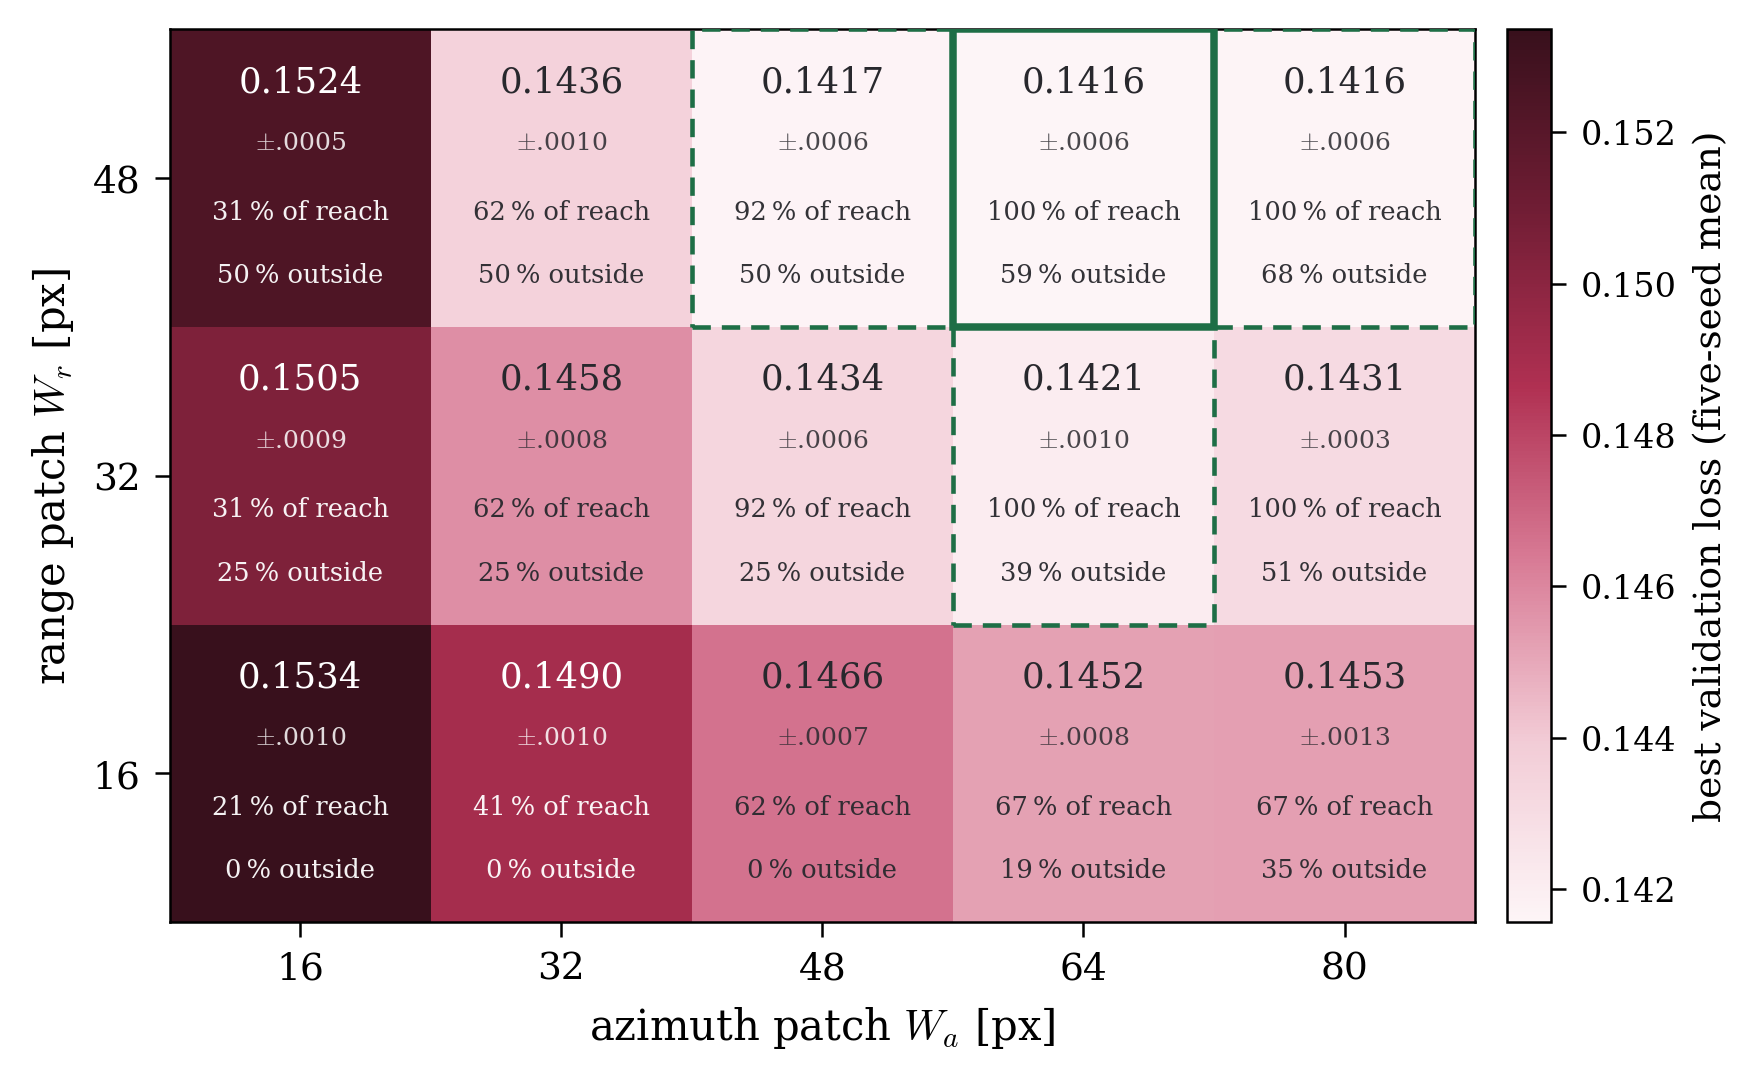
\includegraphics[width=0.56\linewidth]{../figures/K2/Patch/patch_sweep_loss_heatmap.png}
  \par\vspace{4pt}
  {\scriptsize
  \setlength{\tabcolsep}{6pt}
  \begin{tabular}{@{}lll@{}}
    \toprule
                 & registered  & observed \\
    \midrule
    azimuth knee & $2w_a = 52$ & $\mathbf{48}$--$\mathbf{64}$, flat past $48$ \\
    \addlinespace[2pt]
    range knee   & $2w_r = 24$ & $\mathbf{32}$; $\le 0.002$ left to $48$ \\
    \bottomrule
  \end{tabular}}
  \par\vspace{4pt}
  \parbox{0.82\textwidth}{\scriptsize\color{soft} \textbf{runs}: patch $W_a{\times}W_r$ $=$ cell, all else fixed (full input stack, $26{\times}12$ boxcar labels); five seeded replicas per cell, cell $=$ mean best val loss $\pm$ seed std. \textcolor{good}{Green} $=$ best cell, dashed $=$ inside its combined seed noise. \% of reach $=$ share of the centred $2w_a{\times}2w_r$ box ($52{\times}24$) the patch covers; \% outside $=$ share of the patch beyond that box. The residual range drift past its reach clears seed noise at some $W_a$ --- an order below the azimuth climb.\par}
\end{frame}

% ---------------------------------------------------------------- 24d The price of reach
\begin{frame}{The price of reach --- one grid against a pyramid}
  \setlength{\abovedisplayskip}{3pt}
  \setlength{\belowdisplayskip}{3pt}
  \small
  \begin{columns}[T]
    \begin{column}{0.59\textwidth}
      \begin{minipage}[t]{0.43\linewidth}
        \centering
        \textbf{The trunk --- one grid.}
        \[
          \begin{gathered}
            r \;=\; 1 + 2B(k{-}1)\\
            {\color{soft}\scriptstyle +\,2(k{-}1)\ \text{per block}}\\[5pt]
            P \;\propto\; B\,k^{2}m^{2}\\
            {\color{soft}\scriptstyle \text{capacity pinned}}\\[5pt]
            m \;\propto\; \sqrt{P/B}\vphantom{\tfrac{k^{2}m_{\ell}^{2}}{4^{\ell}}}\\
            {\color{soft}\scriptstyle \text{depth paid in width}}
          \end{gathered}
        \]
        \par\vspace{0.06cm}
        \begin{tikzpicture}
          \useasboundingbox (-0.68,-1.128) rectangle (0.68,1.128);
          \draw[black!7, step=0.08] (-0.68,-0.68) grid (0.68,0.68);
          \fill[accent!14] (-0.52,-0.24) rectangle (0.52,0.24);
          \draw[accent, dashed, thin] (-0.52,-0.24) rectangle (0.52,0.24);
          \node[font=\tiny, text=accent, anchor=south west, inner sep=1pt] at (0.44,0.28) {$B(x)$};
          \draw[ink, thin] (-0.10,-0.10) rectangle (0.10,0.10);
          \draw[ink, thin] (-0.18,-0.18) rectangle (0.18,0.18);
          \draw[ink, thin] (-0.26,-0.26) rectangle (0.26,0.26);
          \draw[ink, thin] (-0.34,-0.34) rectangle (0.34,0.34);
          \fill[ink] (-0.02,-0.02) rectangle (0.02,0.02);
        \end{tikzpicture}\\
        {\tiny\color{soft} four blocks, $+\,2(k{-}1)$ each\par}
      \end{minipage}%
      \begin{minipage}[t]{0.075\linewidth}
        \centering
        \begin{tikzpicture}[baseline=(current bounding box.north)]
          \useasboundingbox (0,0) rectangle (0.55,-4.85);
          \draw[flow] (0,-0.55) -- (0.55,-0.55);
          \draw[flow] (0,-1.66) -- (0.55,-1.66);
          \draw[flow] (0,-2.82) -- (0.55,-2.82);
          \draw[flow] (-0.50,-4.77) -- (1.05,-4.77);
        \end{tikzpicture}
      \end{minipage}%
      \begin{minipage}[t]{0.485\linewidth}
        \centering
        \textbf{The pyramid --- halve, conv.}
        \[
          \begin{gathered}
            r \;=\; 1 + 2(k{-}1)\big(2^{D+1}{-}1\big)\\
            {\color{soft}\scriptstyle 2^{\ell}{\times}\ \text{per station}}\\[5pt]
            m_{\ell} \;=\; 2^{\ell}\,m_{0}\\
            {\color{soft}\scriptstyle \text{width doubles down}}\\[5pt]
            \tfrac{k^{2}m_{\ell}^{2}}{4^{\ell}} \;=\; k^{2}m_{0}^{2}\\
            {\color{soft}\scriptstyle \text{cost per pixel flat}}
          \end{gathered}
        \]
        \begin{tikzpicture}[scale=0.88]
          \useasboundingbox (-1.28,-1.28) rectangle (1.28,1.28);
          \draw[black!7, step=0.08] (-1.28,-1.28) grid (1.28,1.28);
          \fill[accent!14] (-0.52,-0.24) rectangle (0.52,0.24);
          \draw[accent, dashed, thin] (-0.52,-0.24) rectangle (0.52,0.24);
          \draw[ink, thin] (-0.10,-0.10) rectangle (0.10,0.10);
          \draw[ink, thin] (-0.26,-0.26) rectangle (0.26,0.26);
          \draw[ink, thin] (-0.58,-0.58) rectangle (0.58,0.58);
          \draw[ink, thin] (-1.22,-1.22) rectangle (1.22,1.22);
          \fill[ink] (-0.02,-0.02) rectangle (0.02,0.02);
        \end{tikzpicture}\\
        {\tiny\color{soft} four stations, the step doubling\par}
      \end{minipage}
    \end{column}
    \begin{column}{0.375\textwidth}
      \raggedright
      {\scriptsize\color{soft}
       $r$: field side \;$\cdot$\;
       $B$: blocks stacked \;$\cdot$\;
       $m$: width in channels \;$\cdot$\;
       $P$: parameters \;$\cdot$\;
       station $\ell$: the block $\ell$ halvings down, width $m_{\ell}$
       \;$\cdot$\; $D$: deepest station\par}
      \par\smallskip
      \centering
      \begin{tikzpicture}[scale=0.93]
        \draw[-{Stealth[length=1.5mm]}, soft] (0,0) -- (0,4.45);
        \draw[-{Stealth[length=1.5mm]}, soft] (0,0) -- (4.60,0)
          node[anchor=south east, font=\tiny, inner sep=1.5pt] {blocks};
        \node[font=\tiny, text=soft, rotate=90, anchor=south] at (-0.30,2.0)
          {field $r$ [px]};
        \foreach \x/\b in {0.60/2,1.20/4,1.80/6,2.40/8,3.00/10,3.60/12,4.20/14}{
          \draw[soft, thin] (\x,0) -- (\x,-0.05);
          \node[font=\tiny, text=soft, anchor=north] at (\x,-0.06) {\b};}
        \draw[soft, dashed, thin] (0,3.38) -- (4.45,3.38);
        \node[font=\tiny, text=soft, anchor=south west, inner sep=1.5pt] at (0.02,3.39) {$2w_{a}$};
        \draw[ink, semithick] (0,0.065) -- (4.20,3.705);
        \node[font=\tiny, text=ink, anchor=south, inner sep=2pt] at (2.90,2.63) {trunk};
        \fill[good] (0.60,0.585) circle (0.05);
        \node[font=\tiny, text=good, anchor=west, inner sep=2.5pt] at (0.64,0.55) {$9{\times}9$};
        \fill[accent] (2.10,1.885) circle (0.05);
        \node[font=\tiny, text=accent, anchor=north west, inner sep=2pt] at (2.12,1.83) {$29{\times}29$};
        \fill[ink] (3.825,3.38) circle (0.05);
        \node[font=\tiny, text=ink, anchor=north west, inner sep=2.5pt] at (3.72,3.30) {$13$};
        \draw[accent, semithick] (0,0.065) -- (0.30,0.325) -- (0.60,0.845)
          -- (0.90,1.885) -- (1.20,3.965);
        \fill[accent] (0.30,0.325) circle (0.05);
        \fill[accent] (0.60,0.845) circle (0.05);
        \fill[accent] (0.90,1.885) circle (0.05);
        \fill[accent] (1.20,3.965) circle (0.05);
        \node[font=\tiny, text=accent, anchor=west, inner sep=2.5pt] at (1.26,3.965) {$4$ stations};
        \draw[soft, dotted, thin] (0.90,1.885) -- (2.10,1.885);
        \node[font=\tiny, text=soft, anchor=south] at (1.50,1.90) {same $29$};
      \end{tikzpicture}
      \par\smallskip
      \raggedright
      {\scriptsize Encoder stations alone --- the decoder only pushes further.
       Three stations hold the ladder's $29{\times}29$; the fourth passes the
       sweep's reach $2w_{a}$, thirteen full-resolution blocks before the
       trunk does.\par}
    \end{column}
  \end{columns}
\end{frame}

% ---------------------------------------------------------------- 24e Why the U-Net fits
\begin{frame}{One grid per scale --- matching the scales of the interferograms}
  \begin{columns}[c]
    \begin{column}{0.50\textwidth}
      \small
      \textbf{Multi-scale by construction} --- each track pair $(P, S_{n})$
      sees the same relief $z(x)$ at its own fringe rate:
      \par\smallskip
      {\centering
      $\varphi_{n}(x) = \bigl(k_z^{(n)} - k_z^{(P)}\bigr)\, z(x)
        = k_{n}\, z(x), \qquad k_{n} \propto b_{\perp,n}$
      \par}
      \medskip
      {\centering
      \begin{tikzpicture}
        \node[font=\scriptsize, text=soft, anchor=south] at (0.55,0.55) {track pair};
        \node[font=\scriptsize, text=soft, anchor=south] at (2.55,0.55) {its fringes};
        \node[font=\scriptsize, text=soft, anchor=south] at (4.80,0.55) {matching grid};
        \draw[soft, thin] (0.40,0.25) -- (0.40,-3.50);
        \draw[|-|, soft] (0.72,-3.50) -- (0.72,0);
        \node[font=\scriptsize, text=soft, anchor=center] at (1.00,-1.75) {$b_{\perp}$};
        \fill[accent] (0.40,-3.50) circle (0.07);
        \node[font=\scriptsize, text=accent, anchor=north, inner sep=2pt] at (0.40,-3.60) {$P$};
        \fill[ink] (0.40,0) circle (0.06);
        \node[font=\scriptsize, text=soft, anchor=east, inner sep=2pt] at (0.28,0) {$S_{1}$};
        \fill[ink] (0.40,-1.30) circle (0.06);
        \node[font=\scriptsize, text=soft, anchor=east, inner sep=2pt] at (0.28,-1.30) {$S_{2}$};
        \fill[ink] (0.40,-2.60) circle (0.06);
        \node[font=\scriptsize, text=soft, anchor=east, inner sep=2pt] at (0.28,-2.60) {$S_{3}$};
        \fill[black!4] (1.45,-0.35) rectangle (3.65,0.35);
        \foreach \j in {0,...,9}
          \fill[ink!40] (1.45+0.22*\j,-0.35) rectangle ++(0.11,0.70);
        \draw[soft, thin] (1.45,-0.35) rectangle (3.65,0.35);
        \fill[black!4] (1.45,-1.65) rectangle (3.65,-0.95);
        \foreach \j in {0,...,4}
          \fill[ink!40] (1.45+0.44*\j,-1.65) rectangle ++(0.22,0.70);
        \draw[soft, thin] (1.45,-1.65) rectangle (3.65,-0.95);
        \fill[black!4] (1.45,-2.95) rectangle (3.65,-2.25);
        \fill[ink!40] (1.45,-2.95) rectangle ++(0.88,0.70);
        \fill[ink!40] (3.21,-2.95) rectangle (3.65,-2.25);
        \draw[soft, thin] (1.45,-2.95) rectangle (3.65,-2.25);
        \draw[-{Stealth[length=1.5mm]}, soft] (3.78,0) -- (4.10,0);
        \draw[-{Stealth[length=1.5mm]}, soft] (3.78,-1.30) -- (4.10,-1.30);
        \draw[-{Stealth[length=1.5mm]}, soft] (3.78,-2.60) -- (4.10,-2.60);
        \begin{scope}[shift={(4.20,-0.40)}]
          \draw[ink!20, step=0.05] (0,0) grid (1.20,0.80);
          \draw[soft, thin] (0,0) rectangle (1.20,0.80);
        \end{scope}
        \begin{scope}[shift={(4.20,-1.70)}]
          \draw[ink!30, step=0.10] (0,0) grid (1.20,0.80);
          \draw[soft, thin] (0,0) rectangle (1.20,0.80);
        \end{scope}
        \begin{scope}[shift={(4.20,-3.00)}]
          \draw[ink!30, step=0.40] (0,0) grid (1.20,0.80);
          \draw[soft, thin] (0,0) rectangle (1.20,0.80);
        \end{scope}
        \node[font=\scriptsize, text=soft, anchor=north] at (4.80,-0.45) {scale 0};
        \node[font=\scriptsize, text=soft, anchor=north] at (4.80,-1.75) {scale 1};
        \node[font=\scriptsize, text=soft, anchor=north] at (4.80,-3.05) {scale 3};
      \end{tikzpicture}
      \par}
    \end{column}
    \begin{column}{0.46\textwidth}
      \centering
      \begin{tikzpicture}[scale=0.85]
        \node[font=\scriptsize, text=ink, anchor=south] at (0.80,1.32) {U-Net};
        \node[font=\scriptsize, text=ink, anchor=south] at (3.25,1.32) {local CNN};
        \begin{scope}
          \fill[argA!30] (0.40,0.40) rectangle (1.20,0.80);
          \draw[ink!20, step=0.05] (0,0) grid (1.60,1.20);
          \draw[accent, dashed, thin] (0.40,0.40) rectangle (1.20,0.80);
          \draw[soft, thin] (0,0) rectangle (1.60,1.20);
          \node[font=\tiny, text=accent, anchor=south west, inner sep=1pt] at (0.36,0.84) {$B(x)$};
        \end{scope}
        \begin{scope}[shift={(0,-1.70)}]
          \fill[argA!30] (0.40,0.40) rectangle (1.20,0.80);
          \draw[ink!30, step=0.10] (0,0) grid (1.60,1.20);
          \draw[accent, dashed, thin] (0.40,0.40) rectangle (1.20,0.80);
          \draw[soft, thin] (0,0) rectangle (1.60,1.20);
        \end{scope}
        \begin{scope}[shift={(0,-3.40)}]
          \fill[argA!30] (0.40,0.40) rectangle (1.20,0.80);
          \draw[ink!30, step=0.20] (0,0) grid (1.60,1.20);
          \draw[accent, dashed, thin] (0.40,0.40) rectangle (1.20,0.80);
          \draw[soft, thin] (0,0) rectangle (1.60,1.20);
        \end{scope}
        \begin{scope}[shift={(0,-5.10)}]
          \fill[argA!30] (0.40,0.40) rectangle (1.20,0.80);
          \draw[ink!30, step=0.40] (0,0) grid (1.60,1.20);
          \draw[accent, dashed, thin] (0.40,0.40) rectangle (1.20,0.80);
          \draw[soft, thin] (0,0) rectangle (1.60,1.20);
        \end{scope}
        \node[font=\tiny, text=soft, anchor=east, align=right, inner sep=2pt] at (-0.08,0.60) {scale 0\\a value per pixel};
        \node[font=\tiny, text=soft, anchor=east, align=right, inner sep=2pt] at (-0.08,-1.10) {scale 1};
        \node[font=\tiny, text=soft, anchor=east, align=right, inner sep=2pt] at (-0.08,-2.80) {scale 2};
        \node[font=\tiny, text=soft, anchor=east, align=right, inner sep=2pt] at (-0.08,-4.50) {scale 3\\two cells};
        \draw[-{Stealth[length=1.5mm]}, soft] (0.80,0) -- (0.80,-0.50);
        \node[font=\tiny, text=soft, anchor=west, inner sep=2pt] at (0.92,-0.25) {$\div 4$};
        \draw[-{Stealth[length=1.5mm]}, soft] (0.80,-1.70) -- (0.80,-2.20);
        \node[font=\tiny, text=soft, anchor=west, inner sep=2pt] at (0.92,-1.95) {$\div 4$};
        \draw[-{Stealth[length=1.5mm]}, soft] (0.80,-3.40) -- (0.80,-3.90);
        \node[font=\tiny, text=soft, anchor=west, inner sep=2pt] at (0.92,-3.65) {$\div 4$};
        \begin{scope}[shift={(2.45,0)}]
          \fill[argA!30] (0.40,0.40) rectangle (1.20,0.80);
          \draw[ink!20, step=0.05] (0,0) grid (1.60,1.20);
          \draw[accent, dashed, thin] (0.40,0.40) rectangle (1.20,0.80);
          \draw[soft, thin] (0,0) rectangle (1.60,1.20);
        \end{scope}
        \begin{scope}[shift={(2.45,-1.70)}]
          \fill[argA!30] (0.40,0.40) rectangle (1.20,0.80);
          \draw[ink!20, step=0.05] (0,0) grid (1.60,1.20);
          \draw[accent, dashed, thin] (0.40,0.40) rectangle (1.20,0.80);
          \draw[soft, thin] (0,0) rectangle (1.60,1.20);
        \end{scope}
        \begin{scope}[shift={(2.45,-3.40)}]
          \fill[argA!30] (0.40,0.40) rectangle (1.20,0.80);
          \draw[ink!20, step=0.05] (0,0) grid (1.60,1.20);
          \draw[accent, dashed, thin] (0.40,0.40) rectangle (1.20,0.80);
          \draw[soft, thin] (0,0) rectangle (1.60,1.20);
        \end{scope}
        \begin{scope}[shift={(2.45,-5.10)}]
          \fill[argA!30] (0.40,0.40) rectangle (1.20,0.80);
          \draw[ink!20, step=0.05] (0,0) grid (1.60,1.20);
          \draw[accent, dashed, thin] (0.40,0.40) rectangle (1.20,0.80);
          \draw[soft, thin] (0,0) rectangle (1.60,1.20);
          \fill[accent] (0.80,0.60) rectangle (0.85,0.65);
          \node[font=\tiny, text=accent, anchor=north, inner sep=2pt] at (0.82,0.58) {$x$};
        \end{scope}
        \node[font=\tiny, text=soft, anchor=north] at (3.25,-5.15) {scale 0 --- unchanged};
        \draw[-{Stealth[length=1.5mm]}, soft] (3.25,0) -- (3.25,-0.50);
        \node[font=\tiny, text=soft, anchor=west, inner sep=2pt] at (3.37,-0.25) {$\times 1$};
        \draw[-{Stealth[length=1.5mm]}, soft] (3.25,-1.70) -- (3.25,-2.20);
        \node[font=\tiny, text=soft, anchor=west, inner sep=2pt] at (3.37,-1.95) {$\times 1$};
        \draw[-{Stealth[length=1.5mm]}, soft] (3.25,-3.40) -- (3.25,-3.90);
        \node[font=\tiny, text=soft, anchor=west, inner sep=2pt] at (3.37,-3.65) {$\times 1$};
        \draw[-{Stealth[length=1.5mm]}, soft] (4.10,-4.50) -- (4.35,-4.50);
        \foreach \i in {0,1,2,3,4,5,6,7}
          \draw[soft, thin, fill=accent!10] (4.40,-4.96+0.115*\i) rectangle (4.90,-4.845+0.115*\i);
        \node[font=\tiny, text=soft, anchor=north, align=center, inner sep=2pt] at (4.65,-5.02)
          {$m$ channels\\at $x$};
      \end{tikzpicture}
    \end{column}
  \end{columns}
\end{frame}

% ---------------------------------------------------------------- 25 Input ablation: the test
\begin{frame}{Input ablation --- which channels, and how many tracks?}
  \begin{columns}[c]
    \begin{column}{0.43\textwidth}
      \centering
      \begin{tikzpicture}
        \node[font=\tiny\bfseries,text=soft] at (1.15,5.75) {reduced --- 5 tracks};
        \node[font=\tiny\bfseries,text=soft] at (3.75,5.75) {all --- 29 tracks};
        \node[font=\tiny\bfseries,text=soft,rotate=90] at (-0.35,4.675) {$|A|$ only};
        \node[font=\tiny\bfseries,text=soft,rotate=90] at (-0.35,2.725) {$\varphi$ only};
        \node[font=\tiny\bfseries,text=soft,rotate=90] at (-0.35,0.775) {$|A|+\varphi$};
        % row 1: amplitude only
        \begin{scope}[shift={(0,3.9)}]
          \draw[soft,thin,rounded corners=2pt,fill=black!2] (0,0) rectangle (2.3,1.55);
          \foreach \i in {3,2,1} \draw[soft,thin,fill=black!2] (0.3+0.05*\i,0.65+0.05*\i) rectangle ++(0.6,0.6);
          \draw[soft,thin,fill=white] (0.3,0.65) rectangle ++(0.6,0.6);
          \draw[black!8,step=0.15,shift={(0.3,0.65)}] (0,0) grid (0.6,0.6);
          \draw[soft,thin,fill=white] (1.3,0.65) rectangle ++(0.6,0.6);
          \begin{scope} \clip (1.3,0.65) rectangle ++(0.6,0.6); \foreach \r in {0.3,0.42,...,1.3} \draw[black!12,thin] (2.05,0.4) circle (\r); \end{scope}
          \draw[accent,thick] (1.3,0.65) -- ++(0.6,0.6);
          \draw[accent,thick] (1.3,1.25) -- ++(0.6,-0.6);
          \node[font=\tiny,text=soft,anchor=north] at (1.15,0.47) {5 $|A|$, no $\varphi$};
        \end{scope}
        \begin{scope}[shift={(2.6,3.9)}]
          \draw[soft,thin,rounded corners=2pt,fill=black!2] (0,0) rectangle (2.3,1.55);
          \foreach \i in {6,5,4,3,2,1} \draw[soft,thin,fill=black!2] (0.3+0.05*\i,0.57+0.05*\i) rectangle ++(0.6,0.6);
          \draw[soft,thin,fill=white] (0.3,0.57) rectangle ++(0.6,0.6);
          \draw[black!8,step=0.15,shift={(0.3,0.57)}] (0,0) grid (0.6,0.6);
          \draw[soft,thin,fill=white] (1.3,0.65) rectangle ++(0.6,0.6);
          \begin{scope} \clip (1.3,0.65) rectangle ++(0.6,0.6); \foreach \r in {0.3,0.42,...,1.3} \draw[black!12,thin] (2.05,0.4) circle (\r); \end{scope}
          \draw[accent,thick] (1.3,0.65) -- ++(0.6,0.6);
          \draw[accent,thick] (1.3,1.25) -- ++(0.6,-0.6);
          \node[font=\tiny,text=soft,anchor=north] at (1.15,0.47) {29 $|A|$, no $\varphi$};
        \end{scope}
        % row 2: phase only
        \begin{scope}[shift={(0,1.95)}]
          \draw[soft,thin,rounded corners=2pt,fill=black!2] (0,0) rectangle (2.3,1.55);
          \draw[soft,thin,fill=white] (0.3,0.65) rectangle ++(0.6,0.6);
          \draw[black!8,step=0.15,shift={(0.3,0.65)}] (0,0) grid (0.6,0.6);
          \draw[accent,thick] (0.3,0.65) -- ++(0.6,0.6);
          \draw[accent,thick] (0.3,1.25) -- ++(0.6,-0.6);
          \foreach \i in {3,2,1} \draw[soft,thin,fill=black!2] (1.3+0.05*\i,0.65+0.05*\i) rectangle ++(0.6,0.6);
          \draw[soft,thin,fill=white] (1.3,0.65) rectangle ++(0.6,0.6);
          \begin{scope} \clip (1.3,0.65) rectangle ++(0.6,0.6); \foreach \r in {0.3,0.42,...,1.3} \draw[accent!30,thin] (2.05,0.4) circle (\r); \end{scope}
          \node[font=\tiny,text=soft,anchor=north] at (1.15,0.47) {4 $\varphi$, no $|A|$};
        \end{scope}
        \begin{scope}[shift={(2.6,1.95)}]
          \draw[soft,thin,rounded corners=2pt,fill=black!2] (0,0) rectangle (2.3,1.55);
          \draw[soft,thin,fill=white] (0.3,0.65) rectangle ++(0.6,0.6);
          \draw[black!8,step=0.15,shift={(0.3,0.65)}] (0,0) grid (0.6,0.6);
          \draw[accent,thick] (0.3,0.65) -- ++(0.6,0.6);
          \draw[accent,thick] (0.3,1.25) -- ++(0.6,-0.6);
          \foreach \i in {6,5,4,3,2,1} \draw[soft,thin,fill=black!2] (1.3+0.05*\i,0.57+0.05*\i) rectangle ++(0.6,0.6);
          \draw[soft,thin,fill=white] (1.3,0.57) rectangle ++(0.6,0.6);
          \begin{scope} \clip (1.3,0.57) rectangle ++(0.6,0.6); \foreach \r in {0.3,0.42,...,1.3} \draw[accent!30,thin] (2.05,0.32) circle (\r); \end{scope}
          \node[font=\tiny,text=soft,anchor=north] at (1.15,0.47) {28 $\varphi$, no $|A|$};
        \end{scope}
        % row 3: both
        \begin{scope}[shift={(0,0)}]
          \draw[accent!60,thin,rounded corners=2pt,fill=accent!4] (0,0) rectangle (2.3,1.55);
          \foreach \i in {3,2,1} \draw[soft,thin,fill=black!2] (0.3+0.05*\i,0.65+0.05*\i) rectangle ++(0.6,0.6);
          \draw[soft,thin,fill=white] (0.3,0.65) rectangle ++(0.6,0.6);
          \draw[black!8,step=0.15,shift={(0.3,0.65)}] (0,0) grid (0.6,0.6);
          \foreach \i in {3,2,1} \draw[soft,thin,fill=black!2] (1.3+0.05*\i,0.65+0.05*\i) rectangle ++(0.6,0.6);
          \draw[soft,thin,fill=white] (1.3,0.65) rectangle ++(0.6,0.6);
          \begin{scope} \clip (1.3,0.65) rectangle ++(0.6,0.6); \foreach \r in {0.3,0.42,...,1.3} \draw[accent!30,thin] (2.05,0.4) circle (\r); \end{scope}
          \node[font=\tiny,text=soft,anchor=north] at (1.15,0.47) {5 $|A|$ + 4 $\varphi$};
          \node[font=\tiny,text=accent,anchor=north] at (1.15,-0.06) {reference (reduced stack)};
        \end{scope}
        \begin{scope}[shift={(2.6,0)}]
          \draw[soft,thin,rounded corners=2pt,fill=black!2] (0,0) rectangle (2.3,1.55);
          \foreach \i in {6,5,4,3,2,1} \draw[soft,thin,fill=black!2] (0.3+0.05*\i,0.57+0.05*\i) rectangle ++(0.6,0.6);
          \draw[soft,thin,fill=white] (0.3,0.57) rectangle ++(0.6,0.6);
          \draw[black!8,step=0.15,shift={(0.3,0.57)}] (0,0) grid (0.6,0.6);
          \foreach \i in {6,5,4,3,2,1} \draw[soft,thin,fill=black!2] (1.3+0.05*\i,0.57+0.05*\i) rectangle ++(0.6,0.6);
          \draw[soft,thin,fill=white] (1.3,0.57) rectangle ++(0.6,0.6);
          \begin{scope} \clip (1.3,0.57) rectangle ++(0.6,0.6); \foreach \r in {0.3,0.42,...,1.3} \draw[accent!30,thin] (2.05,0.32) circle (\r); \end{scope}
          \node[font=\tiny,text=soft,anchor=north] at (1.15,0.47) {29 $|A|$ + 28 $\varphi$};
          \node[font=\tiny,text=soft,anchor=north] at (1.15,-0.06) {full stack};
        \end{scope}
      \end{tikzpicture}
    \end{column}
    \begin{column}{0.54\textwidth}
      \small
      Theory says the elevation information lives in the \textbf{interferogram
      phase}: amplitudes alone should not determine the profile. But the context
      ladder just showed the network leans on spatial structure --- so two axes,
      crossed:
      \par\smallskip
      \begin{itemize}\setlength{\itemsep}{3pt}
        \item \textbf{The grid}: \emph{which channels} ($|A|$ only / $\varphi$
              only / both) $\times$ \emph{how many tracks} (the reduced 5-track
              selection / all 29). Six retrains of the reference U-Net --- same
              $K{=}2$ target, loss and split, only the input stack changes.
        \item \textbf{H1 --- phase is everything}: strip the phase and
              reconstruction collapses toward nothing usable; amplitude
              diversity cannot buy it back.
        \item \textbf{H2 --- priors carry part of it}: amplitude-only lands in
              between, and 29 $|A|$ closes part of the gap to the reference.
        \item \textbf{H3 --- tracks pay everywhere}: if tracks are information,
              every modality should improve reduced $\to$ all; the open question
              is whether diversity can \emph{substitute} for a missing modality.
      \end{itemize}
    \end{column}
  \end{columns}
\end{frame}

% ---------------------------------------------------------------- 25b Input ablation: the verdict
\begin{frame}{The verdict --- every channel pays on the curve, phase still places the scatterers}
    \centering
  \scriptsize
  \renewcommand{\arraystretch}{0.98}
  \setlength{\tabcolsep}{2.5pt}
  \renewcommand{\seedtag}{ctxA}
  \begin{tabular}{@{}l cc cc !{\hspace{3pt}} cc@{}}
    \toprule
    & \multicolumn{2}{c}{$|A|$ only} & \multicolumn{2}{c}{$\varphi$ only} & \multicolumn{2}{c@{}}{$|A|+\varphi$} \\
    \cmidrule(lr){2-3}\cmidrule(lr){4-5}\cmidrule(l){6-7}
    metric & red. & all & red. & all & red. & all \\
    \midrule
    \multicolumn{7}{@{}l}{\emph{training (validation)}} \\
    val loss $\downarrow$ & \seedpm{0.179}{.001} & \seedpm{0.164}{.002} & \seedpm{0.162}{.001} & \seedpm{0.137}{.002} & \seedpm{0.142}{.001} & \seedpm{\hlval{good}{\textbf{0.122}}}{.000} \\
    \addlinespace
    \multicolumn{7}{@{}l}{\emph{reconstruction (curve)}} \\
    curve $R^2$ $\uparrow$ & \seedpm{0.369}{.014} & \seedpm{0.437}{.010} & \seedpm{0.409}{.018} & \seedpm{0.503}{.007} & \seedpm{0.569}{.008} & \seedpm{\hlval{good}{\textbf{0.667}}}{.015} \\
    curve MAE $\downarrow$ & \seedpm{0.066}{.001} & \seedpm{0.060}{.001} & \seedpm{0.059}{.002} & \seedpm{0.051}{.001} & \seedpm{0.050}{.001} & \seedpm{\textbf{0.043}}{.001} \\
    PSNR [dB] $\uparrow$  & \seedpm{48.7}{.1} & \seedpm{49.2}{.1} & \seedpm{48.9}{.1} & \seedpm{49.7}{.1} & \seedpm{50.3}{.1} & \seedpm{\textbf{51.4}}{.2} \\
    SSIM elev $\uparrow$  & \seedpm{0.946}{.001} & \seedpm{0.951}{.001} & \seedpm{0.952}{.001} & \seedpm{0.959}{.001} & \seedpm{0.959}{.001} & \seedpm{0.963}{.001} \\
    SSIM range $\uparrow$ & \seedpm{0.901}{.001} & \seedpm{0.911}{.002} & \seedpm{0.916}{.002} & \seedpm{0.927}{.002} & \seedpm{0.926}{.002} & \seedpm{0.933}{.001} \\
    SSIM azim $\uparrow$  & \seedpm{0.925}{.000} & \seedpm{0.933}{.001} & \seedpm{0.936}{.002} & \seedpm{0.946}{.001} & \seedpm{0.946}{.001} & \seedpm{0.953}{.001} \\
    profile cos med\,$\uparrow$ & \seedpm{0.665}{.020} & \seedpm{0.737}{.017} & \seedpm{0.912}{.012} & \seedpm{\textbf{0.931}}{.009} & \seedpm{0.850}{.024} & \seedpm{0.890}{.012} \\
    \addlinespace
    \multicolumn{7}{@{}l}{\emph{detection (matched)}} \\
    precision $\uparrow$   & \seedpm{0.758}{.008} & \seedpm{0.785}{.009} & \seedpm{0.830}{.007} & \seedpm{\textbf{0.853}}{.008} & \seedpm{0.821}{.008} & \seedpm{0.839}{.005} \\
    recall $\uparrow$      & \seedpm{0.652}{.027} & \seedpm{0.679}{.028} & \seedpm{\hlval{good}{\textbf{0.817}}}{.021} & \seedpm{0.765}{.038} & \seedpm{0.641}{.029} & \seedpm{\hlval{accent}{0.636}}{.024} \\
    matched F1 $\uparrow$  & \seedpm{0.701}{.019} & \seedpm{0.728}{.020} & \seedpm{\hlval{good}{\textbf{0.823}}}{.012} & \seedpm{0.806}{.024} & \seedpm{0.720}{.020} & \seedpm{0.723}{.017} \\
    count exact $\uparrow$ & \seedpm{0.609}{.034} & \seedpm{0.633}{.035} & \seedpm{\hlval{good}{\textbf{0.802}}}{.029} & \seedpm{0.741}{.048} & \seedpm{0.595}{.034} & \seedpm{0.591}{.033} \\
    peak err med $\downarrow$ & \seedpm{1.48}{.30} & \seedpm{1.34}{.00} & \seedpm{\textbf{0.67}}{.00} & \seedpm{\textbf{0.67}}{.00} & \seedpm{0.81}{.30} & \seedpm{0.81}{.30} \\
    peak err p95 $\downarrow$ & \seedpm{15.6}{.3} & \seedpm{15.3}{.3} & \seedpm{\textbf{11.7}}{1.9} & \seedpm{14.0}{.3} & \seedpm{15.4}{.5} & \seedpm{15.2}{.4} \\
    \bottomrule
  \end{tabular}
  \par\vspace{3pt}
  \parbox{0.82\textwidth}{\tiny\color{soft} \textbf{runs}: UNet $\cdot$ conv $\cdot$ sorted-GT $\cdot$ $K{=}2$ $\cdot$ param-MSE $\cdot$ presence none $\cdot$ full norm ladder $\cdot$ hv flips $\cdot$ patch $64{\times}32$ (input = column); five seeded replicas per arm, cells mean $\pm$ seed std; held-out test, $5.0$\,M px. red.\ $=$ 5 tracks (5 $|A|$ / 4 $\varphi$); all $=$ 29 tracks (29 $|A|$ / 28 $\varphi$). \textbf{bold} $=$ best in row, marked only where best and worst differ by more than $5\%$; \textcolor{good}{green} $=$ the full-stack curve peak and the phase detection wins, \textcolor{accent}{red} $=$ amplitude diluting recall; matched $=$ Hungarian pairing. Peak err med/p95: per-pixel peak-error distribution; profile cos med: median per-pixel cosine to the GT profile.\par}
    

\end{frame}

% ---------------------------------------------------------------- 25c Input ablation by scatterer count
\begin{frame}{Input ablation by scatterer count --- each parameter reads its own modality}
    \centering
  \scriptsize
  \renewcommand{\arraystretch}{1.04}
  \setlength{\tabcolsep}{2.5pt}
  \renewcommand{\seedtag}{ctxB}
  \begin{tabular}{@{}l cc cc !{\hspace{3pt}} cc@{}}
    \toprule
    & \multicolumn{2}{c}{$|A|$ only} & \multicolumn{2}{c}{$\varphi$ only} & \multicolumn{2}{c@{}}{$|A|+\varphi$} \\
    \cmidrule(lr){2-3}\cmidrule(lr){4-5}\cmidrule(l){6-7}
    metric & red. & all & red. & all & red. & all \\
    \midrule
    matched precision $\uparrow$ & \seedpm{0.758}{.008} & \seedpm{0.785}{.009} & \seedpm{0.830}{.007} & \seedpm{\textbf{0.853}}{.008} & \seedpm{0.821}{.008} & \seedpm{0.839}{.005} \\
    \quad $k{=}1$                & \seedpm{0.803}{.012} & \seedpm{0.821}{.011} & \seedpm{0.875}{.007} & \seedpm{\textbf{0.890}}{.009} & \seedpm{0.853}{.008} & \seedpm{0.867}{.011} \\
    \quad $k{=}2$                & \seedpm{0.696}{.009} & \seedpm{0.734}{.009} & \seedpm{0.761}{.012} & \seedpm{0.803}{.008} & \seedpm{0.782}{.007} & \seedpm{\textbf{0.806}}{.007} \\
    \addlinespace
    matched recall $\uparrow$    & \seedpm{0.652}{.027} & \seedpm{0.679}{.028} & \seedpm{\hlval{good}{\textbf{0.817}}}{.021} & \seedpm{0.765}{.038} & \seedpm{0.641}{.029} & \seedpm{\hlval{accent}{0.636}}{.024} \\
    \quad $k{=}1$                & \seedpm{0.684}{.046} & \seedpm{0.704}{.047} & \seedpm{\hlval{good}{\textbf{0.882}}}{.040} & \seedpm{0.779}{.065} & \seedpm{0.620}{.046} & \seedpm{0.593}{.043} \\
    \quad $k{=}2$                & \seedpm{0.606}{.009} & \seedpm{0.643}{.007} & \seedpm{0.725}{.009} & \seedpm{\hlval{good}{\textbf{0.745}}}{.003} & \seedpm{0.672}{.008} & \seedpm{0.698}{.008} \\
    \addlinespace
    count acc\,$\mid$\,pred $k{=}1$\,$\uparrow$ & \seedpm{0.961}{.004} & \seedpm{0.963}{.004} & \seedpm{0.969}{.005} & \seedpm{0.964}{.003} & \seedpm{0.948}{.007} & \seedpm{0.959}{.002} \\
    count acc\,$\mid$\,pred $k{=}2$\,$\uparrow$ & \seedpm{0.646}{.003} & \seedpm{0.665}{.007} & \seedpm{0.724}{.007} & \seedpm{\hlval{good}{\textbf{0.770}}}{.005} & \seedpm{0.733}{.010} & \seedpm{0.767}{.007} \\
    \addlinespace
    matched $\mu$ MAE $\downarrow$ & \seedpm{2.95}{.09} & \seedpm{2.65}{.08} & \seedpm{2.29}{.08} & \seedpm{\textbf{2.04}}{.12} & \seedpm{2.30}{.08} & \seedpm{2.15}{.06} \\
    \quad $k{=}1$                & \seedpm{1.25}{.05} & \seedpm{1.03}{.04} & \seedpm{0.55}{.05} & \seedpm{\hlval{good}{\textbf{0.51}}}{.02} & \seedpm{0.59}{.04} & \seedpm{0.52}{.02} \\
    \addlinespace[2pt]
    \quad $k{=}2$                & \seedpm{4.88}{.08} & \seedpm{4.52}{.06} & \seedpm{4.58}{.15} & \seedpm{3.86}{.12} & \seedpm{4.05}{.08} & \seedpm{\textbf{3.74}}{.06} \\
    \addlinespace
    matched $\sigma$ MAE $\downarrow$ & \seedpm{0.97}{.03} & \seedpm{0.91}{.03} & \seedpm{0.89}{.04} & \seedpm{\textbf{0.79}}{.05} & \seedpm{0.87}{.03} & \seedpm{0.80}{.03} \\
    \quad $k{=}1$                & \seedpm{0.29}{.02} & \seedpm{0.26}{.01} & \seedpm{0.24}{.01} & \seedpm{\textbf{0.20}}{.01} & \seedpm{0.25}{.01} & \seedpm{0.21}{.01} \\
    \quad $k{=}2$                & \seedpm{1.74}{.01} & \seedpm{1.64}{.01} & \seedpm{1.76}{.05} & \seedpm{1.51}{.05} & \seedpm{1.51}{.01} & \seedpm{\textbf{1.38}}{.01} \\
    \addlinespace
    matched $a$ MAE $\downarrow$ & \seedpm{0.369}{.017} & \seedpm{0.356}{.015} & \seedpm{\hlval{accent}{0.464}}{.009} & \seedpm{\hlval{accent}{0.446}}{.025} & \seedpm{0.374}{.026} & \seedpm{\textbf{0.346}}{.012} \\
    \quad $k{=}1$                & \seedpm{0.164}{.015} & \seedpm{\textbf{0.161}}{.010} & \seedpm{0.233}{.010} & \seedpm{0.234}{.021} & \seedpm{\textbf{0.161}}{.017} & \seedpm{0.165}{.016} \\
    \quad $k{=}2$                & \seedpm{0.601}{.007} & \seedpm{0.579}{.027} & \seedpm{0.771}{.013} & \seedpm{0.698}{.011} & \seedpm{0.593}{.022} & \seedpm{\textbf{0.524}}{.007} \\
    \bottomrule
  \end{tabular}
  \par\vspace{3pt}
  \parbox{0.82\textwidth}{\tiny\color{soft} \textbf{runs}: UNet $\cdot$ conv $\cdot$ sorted-GT $\cdot$ $K{=}2$ $\cdot$ param-MSE $\cdot$ presence none $\cdot$ full norm ladder $\cdot$ hv flips $\cdot$ patch $64{\times}32$ (input = column); held-out test, cells mean $\pm$ seed std over five seeded replicas; $k$ $=$ true scatterer count of the pixel. red.\ $=$ 5 tracks, all $=$ 29 tracks. \textbf{bold} $=$ best in row, marked only where best and worst differ by more than $5\%$; \textcolor{good}{green} $=$ detection and position living in the phase, \textcolor{accent}{red} $=$ amplitude error without the $|A|$ channels. Precision rewards under-prediction --- rank on recall. count acc $\mid$ pred $k$: share of pixels claiming exactly $k$ scatterers whose true count is $k$. $\mu$, $\sigma$ in elevation units; $a$ in linear amplitude.\par}
    

\end{frame}

% ---------------------------------------------------------------- 25d Input ablation: predicted stats vs GT
\begin{frame}{Input ablation, predicted statistics vs the GT --- phase fires the slots, the full stack calibrates layover}
    \centering
  \scriptsize
  \renewcommand{\arraystretch}{0.90}
  \setlength{\tabcolsep}{2.5pt}
  \renewcommand{\seedtag}{ctxC}
  \begin{tabular}{@{}l !{\color{white}\vrule width 1.2pt} c !{\color{white}\vrule width 1.2pt} cc cc !{\hspace{1pt}} cc@{}}
    \toprule
    & & \multicolumn{2}{c}{$|A|$ only} & \multicolumn{2}{c}{$\varphi$ only} & \multicolumn{2}{c@{}}{$|A|+\varphi$} \\
    \cmidrule(lr){3-4}\cmidrule(lr){5-6}\cmidrule(l){7-8}
    prediction mean & \textcolor{good}{GT} & red. & all & red. & all & red. & all \\
    \midrule
    \multicolumn{8}{@{}l}{\textcolor{soft}{\emph{slot 0 --- strongest scatterer; GT-active on every pixel}}} \\
    \quad active frac         & 1.00    & \seedpm{0.74}{.03} & \seedpm{0.75}{.04} & \seedpm{\hlval{good}{\textbf{0.90}}}{.03} & \seedpm{0.82}{.05} & \seedpm{0.69}{.03} & \seedpm{0.67}{.03} \\
    \quad $a$ --- active      & 0.77    & \seedpm{0.85}{.03} & \seedpm{0.83}{.04} & \seedpm{0.71}{.04} & \seedpm{\textbf{0.72}}{.02} & \seedpm{0.90}{.03} & \seedpm{0.92}{.04} \\
    \quad $\mu$ --- active    & $-4.89$ & \seedpm{$-4.03$}{.10} & \seedpm{$-4.15$}{.17} & \seedpm{$-4.29$}{.05} & \seedpm{\textbf{$-4.52$}}{.08} & \seedpm{$-3.92$}{.10} & \seedpm{$-4.16$}{.09} \\
    \quad $\sigma$ --- active & 1.76    & \seedpm{1.49}{.04} & \seedpm{1.50}{.03} & \seedpm{1.41}{.05} & \seedpm{1.59}{.06} & \seedpm{1.48}{.05} & \seedpm{\textbf{1.65}}{.04} \\
    \addlinespace[1.5pt]
    \multicolumn{8}{@{}l}{\textcolor{soft}{\emph{slot 1 --- second scatterer; GT-active on 26\% of pixels}}} \\
    \quad active frac         & 0.260 & \seedpm{0.346}{.003} & \seedpm{0.338}{.006} & \seedpm{0.338}{.006} & \seedpm{0.308}{.004} & \seedpm{0.299}{.006} & \seedpm{\hlval{good}{\textbf{0.289}}}{.004} \\
    \quad $a$ --- active      & 1.43  & \seedpm{1.05}{.02} & \seedpm{1.08}{.05} & \seedpm{1.05}{.05} & \seedpm{1.08}{.03} & \seedpm{1.04}{.03} & \seedpm{\hlval{good}{\textbf{1.15}}}{.01} \\
    \quad $a$ --- inact.      & 0.00  & \seedpm{0.68}{.01} & \seedpm{0.64}{.03} & \seedpm{0.44}{.04} & \seedpm{0.48}{.01} & \seedpm{\textbf{0.42}}{.01} & \seedpm{0.49}{.03} \\
    \quad $\mu$ --- active    & 11.34 & \seedpm{9.73}{.46} & \seedpm{9.60}{.61} & \seedpm{10.20}{.14} & \seedpm{10.25}{.51} & \seedpm{10.09}{.33} & \seedpm{\hlval{good}{\textbf{10.79}}}{.29} \\
    \quad $\mu$ --- inact.    & ---   & \seedpm{4.04}{.38} & \seedpm{2.72}{.33} & \seedpm{3.51}{.35} & \seedpm{2.55}{.28} & \seedpm{4.09}{.31} & \seedpm{3.71}{.21} \\
    \quad $\sigma$ --- active & 3.53  & \seedpm{3.10}{.03} & \seedpm{3.12}{.05} & \seedpm{2.99}{.02} & \seedpm{3.11}{.05} & \seedpm{2.94}{.05} & \seedpm{\hlval{good}{\textbf{3.18}}}{.03} \\
    \quad $\sigma$ --- inact. & ---   & \seedpm{2.47}{.02} & \seedpm{2.19}{.04} & \seedpm{1.91}{.02} & \seedpm{1.86}{.02} & \seedpm{1.87}{.03} & \seedpm{1.81}{.02} \\
    \addlinespace[1.5pt]
    \multicolumn{8}{@{}l}{\textcolor{soft}{\emph{distribution width --- std over GT-active pixels}}} \\
    \quad $a$ --- slot 0      & 1.48  & \seedpm{1.15}{.02} & \seedpm{1.16}{.05} & \seedpm{1.00}{.06} & \seedpm{1.00}{.02} & \seedpm{1.17}{.03} & \seedpm{\textbf{1.19}}{.01} \\
    \quad $\mu$ --- slot 0    & 3.30  & \seedpm{1.73}{.08} & \seedpm{1.91}{.07} & \seedpm{2.11}{.07} & \seedpm{\textbf{2.33}}{.10} & \seedpm{1.99}{.07} & \seedpm{2.24}{.07} \\
    \quad $\sigma$ --- slot 0 & 2.84  & \seedpm{0.83}{.01} & \seedpm{0.91}{.02} & \seedpm{1.01}{.05} & \seedpm{\textbf{1.35}}{.07} & \seedpm{0.95}{.03} & \seedpm{1.28}{.01} \\
    \quad $a$ --- slot 1      & 1.45  & \seedpm{0.77}{.02} & \seedpm{0.83}{.05} & \seedpm{0.86}{.04} & \seedpm{0.87}{.02} & \seedpm{0.83}{.04} & \seedpm{\textbf{0.89}}{.01} \\
    \quad $\mu$ --- slot 1    & 16.24 & \seedpm{7.14}{.29} & \seedpm{7.74}{.36} & \seedpm{9.37}{.31} & \seedpm{\textbf{10.90}}{.75} & \seedpm{8.72}{.18} & \seedpm{10.06}{.27} \\
    \quad $\sigma$ --- slot 1 & 4.01  & \seedpm{0.80}{.03} & \seedpm{0.92}{.04} & \seedpm{1.08}{.02} & \seedpm{1.33}{.04} & \seedpm{1.07}{.02} & \seedpm{\textbf{1.34}}{.03} \\
    \bottomrule
  \end{tabular}
  \par\vspace{3pt}
  \parbox{0.82\textwidth}{\tiny\color{soft} \textbf{runs}: UNet $\cdot$ conv $\cdot$ sorted-GT $\cdot$ $K{=}2$ $\cdot$ param-MSE $\cdot$ presence none $\cdot$ full norm ladder $\cdot$ hv flips $\cdot$ patch $64{\times}32$ (input = column); five seeded replicas per arm, cells mean $\pm$ seed std; means conditioned on the slot's GT activity mask. red.\ $=$ 5 tracks, all $=$ 29 tracks. \textbf{bold} $=$ closest to the \textcolor{good}{GT} column, marked only where best and worst differ by more than $5\%$; \textcolor{good}{green} $=$ phase firing the slots and the full-stack slot-1 calibration. Inactive GT slots define no $\mu$/$\sigma$ reference (---). Width rows: std of the prediction over GT-active pixels vs the GT's own std. $\mu$, $\sigma$ in elevation units; $a$ in linear amplitude.\par}
    

\end{frame}
